\documentclass[12pt,english]{article}

%%%%%%%%%%%%%%%%%%%%%%%%%
%% SEC: PACKAGEs MAIN  %%
%%%%%%%%%%%%%%%%%%%%%%%%%
\usepackage{mathpazo}
\usepackage{eulervm}
\usepackage{amsmath}
\usepackage{amssymb}
\usepackage[utf8]{inputenc}
\usepackage[T1]{fontenc}
\usepackage{color}
% \usepackage[monochrome]{xcolor}
\usepackage{babel}
\usepackage{csquotes}
\usepackage{setspace}
\usepackage{graphicx}
\usepackage{booktabs,dcolumn}
\usepackage{array}
\usepackage{multirow}
\usepackage[font=singlespacing, skip=3pt]{caption}
\usepackage[usenames,dvipsnames,svgnames,table]{xcolor}
%\usepackage[usenames,dvipsnames,svgnames,table,monochrome]{xcolor} % test black and white color results, 2018-11-21 08:48
\usepackage{float}
\usepackage[export]{adjustbox}[2011/08/13]
\usepackage{enumitem}
\usepackage{tikz}
\usepackage{subfig}
\usepackage{float}
%\usepackage[nolists, tablesfirst, nomarkers]{endfloat}
% \usepackage[unicode=true,pdfusetitle,
%  bookmarks=true,bookmarksnumbered=false,bookmarksopen=false,
%  breaklinks=false,pdfborder={0 0 1},backref=false,colorlinks=false]
%  {hyperref}
\usepackage[colorlinks=true, linkcolor=blue, citecolor=blue, plainpages=false, pdfpagelabels=true, urlcolor=blue]{hyperref}
\usepackage{geometry}
\usepackage{ragged2e}

%%%%%%%%%%%%%%%%%%%%%%%%%
%% SEC: Indentation  %%
%%%%%%%%%%%%%%%%%%%%%%%%%
\geometry{
	a4paper,
	noheadfoot=true,
	left=1.0in,
	right=1.0in,
	top=1.0in,
	bottom=1.0in,
}
\setlength{\parindent}{15pt}
\makeatletter
%\doublespacing
\onehalfspacing
\date{Summer 2020}
%\date{\today}
%\date{}

%%%%%%%%%%%%%%%%%%%%%%%%%
%% SEC: new commands  %%
%%%%%%%%%%%%%%%%%%%%%%%%%
%\exhyphenpenalty=10000\hyphenpenalty=10000
\newcommand\invisiblesection[1]{%
	\refstepcounter{section}%
	\addcontentsline{toc}{section}{\protect\numberline{\thesection}#1}%
	\sectionmark{#1}}

\newcommand{\rowgroup}[1]{\hspace{-0.5em}#1}

\newcommand*\samethanks[1][\value{footnote}]{\footnotemark[#1]}
\newcommand{\sym}[1]{\ifmmode^{#1}\else\(^{#1}\)\fi}


%%%%%%%%%%%%%%%%%%%%%%%%
%% SEC: Footer  %%
%%%%%%%%%%%%%%%%%%%%%%%%
\usepackage{calc}
\setlength{\footskip}{\paperheight
	-(1in+\voffset+\topmargin+\headheight+\headsep+\textheight)
	-0.75in}


% %%%%%%%%%%%%%%%%%%%%%%%%%%%%%% User specified LaTeX commands.
% \usepackage{setspace}
% \usepackage{parskip}
% \usepackage{float}
%
% \usepackage{graphicx}
% \usepackage{booktabs,dcolumn}
% \usepackage[font=singlespacing,skip=5pt]{caption}
%
% \usepackage[usenames,dvipsnames,svgnames,table]{xcolor}
%
% \usepackage[margin=1in]{geometry}
%
%
% \usepackage{mathpazo} % add possibly `sc` and `osf` options
% \usepackage{eulervm}
%
% \usepackage[bottom]{footmisc}
%
% %%%%%%%%%%%%%%%%%%%%%%%%%%%%%5
% %% Recent addition
% %%%%%%%%%%%%%%%%%%%%%%%%%%%%%5
\usepackage{mathtools} % for \coloneqq, 2018-08-27 10:49
\usepackage{accents} % for double dilta 2018-11-16 17:49
\newcommand{\dbtilde}[1]{\accentset{\approx}{#1}}
\usepackage[outdir=./]{epstopdf} % to include eps files, 2018-11-19 08:59
% 2018-11-21 08:51 black and white testing of eps graphs
\usepackage{xspace} % 2018-11-22 15:07 added for newcommand space problem

% 2018-12-03 11:28: color box to generate legend for equilibrium results plots
\usepackage[most]{tcolorbox}
% \definecolor{background}{HTML}{FCF9EE}
% \definecolor{background}{HTML}{FFFFFF}
\definecolor{background}{HTML}{f2f2f2}
% \definecolor{linecolor}{HTML}{581810}
\definecolor{linecolor}{HTML}{000000}
\AtBeginEnvironment{tcolorbox}{\scriptsize}

% For capitalization Needs
\usepackage{mfirstuc}

% More Math
% \usepackage{pgfmath}

% 2018-12-30 13:02
\usetikzlibrary{positioning}

% 2019-01-02 19:32, to allow for multiple footnotes together
\usepackage[multiple]{footmisc}

% 2019-01-07 11:34, to allow for calculations
\usepackage{calculator}

%
%
% \setlength{\parskip}{1mm}
%
% \setlength{\parindent}{20pt}
% \large
% \date{\today}
%
% \onehalfspace
%
% \fboxsep=2mm%padding thickness
% \fboxrule=0.5pt%border thickness
%
% %\exhyphenpenalty=10000\hyphenpenalty=10000

%%%%%%%%%%%%%%%%%%%%%%%%%%%%%%%%%%%%%%%%%%%%%%%%%%%%%%%%%%%%%%%%%%%%%%
%%% Table formatting, 2018-08-27 16:57, for equilibrium solution table
%%%%%%%%%%%%%%%%%%%%%%%%%%%%%%%%%%%%%%%%%%%%%%%%%%%%%%%%%%%%%%%%%%%%%%

\usepackage{array}
\usepackage{makecell}
\renewcommand\theadalign{bc}
\renewcommand\theadfont{\bfseries}
\renewcommand\theadgape{\Gape[4pt]}
\renewcommand\cellgape{\Gape[4pt]}

\newcolumntype{L}[1]{>{\raggedright\let\newline\\\arraybackslash\hspace{0pt}}m{#1}}
\newcolumntype{C}[1]{>{\centering\let\newline\\\arraybackslash\hspace{0pt}}m{#1}}
\newcolumntype{R}[1]{>{\raggedleft\let\newline\\\arraybackslash\hspace{0pt}}m{#1}}


%%%%%%%%%%%%%%%%%%%%%%%%%%%%%%%%%%%%%%%%%%%%%%%%%%%%%%%%%%%%%%%%%%%%%%
%%% Common Section Headings
%%%%%%%%%%%%%%%%%%%%%%%%%%%%%%%%%%%%%%%%%%%%%%%%%%%%%%%%%%%%%%%%%%%%%%

\renewcommand{\section}{\@startsection {section}{1}{\z@}%
             {-3.5ex \@plus -1ex \@minus -.2ex}%
             {2.3ex \@plus .2ex}%
             {\normalfont\Large\scshape\bfseries}}

\renewcommand{\subsection}{\@startsection{subsection}{2}{\z@}%
             {-3.25ex\@plus -1ex \@minus -.2ex}%
             {1.5ex \@plus .2ex}%
             {\normalfont\large\scshape\bfseries}}

\renewcommand{\subsubsection}{\@startsection{subsubsection}{2}{\z@}%
             {-3.25ex\@plus -1ex \@minus -.2ex}%
             {1.5ex \@plus .2ex}%
             {\normalfont\normalsize}}

%%%%%%%%%%%%%%%%%%%%%%%%%%%%%%%%%%%%%%%%%%%%%%%%%%%%%%%%%%%%%%%%%%%%%%
%%% Edit Notes
%%%%%%%%%%%%%%%%%%%%%%%%%%%%%%%%%%%%%%%%%%%%%%%%%%%%%%%%%%%%%%%%%%%%%%

\newcommand{\EDIT}[2]{\textit{#1 (\textcolor{red}{\textbf{EDIT}} #2)}}
\newcommand{\REFE}[1]{\textit{#1 (\textcolor{blue}{\textbf{R}})}}

%%%%%%%%%%%%%%%%%%%%%%%%
%% SEC: Bibliography %%
%%%%%%%%%%%%%%%%%%%%%%%%
\usepackage[authordate,
backend=bibtex,
doi=false,
isbn=false,
sorting=nyt,
maxbibnames=10,
maxcitenames=3,
sortcites=False]{biblatex-chicago}


% \bibliography{../_bib/ref_one, ../_bib/ref_two, ../_bib/ref_three, ../_bib/ref_four, ../_bib/ref_five}

\AtEveryBibitem{\clearlist{note}\clearlist{language}\clearlist{issn}} % clears issn
\AtEveryBibitem{%
	\ifentrytype{online}{%
		\clearfield{urlyear}
		\clearfield{urlmonth}
		\clearfield{urlday}
		\clearfield{note}
		\clearlist{language}
	}{%
		\clearfield{eprint}%
		\clearfield{url}%
		\clearfield{urlyear}
		\clearfield{urlmonth}
		\clearfield{urlday}
		\clearfield{note}
		\clearlist{language}
	}
}

% \renewcommand*{\bibfont}{\small}

\bibliography{bib/ref_one, bib/ref_two}

\makeatother

\begin{document}

\title{Will Religious People Listen to Science?}

\author{Yeabin Moon \thanks{See \href{https://fanwangecon.github.io/Tex4Econ/}{Tex4Econ} for more latex examples.} \\ \textit{Research Proposal}}


\maketitle
\begin{abstract}
\singlespacing filled\end{abstract}
\vfill
\pagebreak{}

\section{Research Log}
\subsection{Identify Religious Worship places} 

First of all, using NAICS code, select religious POI in California. The number of POI in raw file is 18510. 

It is not clear whether the selected POI is serving as a worship place. The main treatment is whether one attends the services or not, and hence it is important to distinguish the worship places from other purposes of religious POIs. The idea to find worship places is that most religious gatherings or services happen either Friday, Saturday or Sunday. Hence, we use Monthly Places Patterns series and figure out the most popular days in 2019 for all religious POIs, and select the POIs having Friday, Saturday or Sunday as the most popular days. The number of POIs is 11825.

\subsection{Classify the  places} 

The next step is to figure out the size of the POIs and whether they closes during the pandemic. Two things are worth to be mentioned. First, if the number of unique visitors are less than 4, SafeGraph does not reveal where the visitors' home census block because of privacy issues. The main point is how the visitors' behavior, not the religious places, we only keep the POIs having more than 4 unique visitors in 2020. Second, the baseline periods (prior to pandemic) are January and February. The pandemic period starts at March 6th. On March 6, San Francisco warns vulnerable residents to avoid outings and larger groups, businesses to suspend non-essential travel and consider telecommuting, and cancellation of all non-essential large events, and the city began restricting event size a few days later. By March 16, six Bay Area counties became the first in the nation to announce shelter-in-place orders and on March 19, the State of California became the first to mandate a state-wide order. Hence, to construct the baseline behavior we use 8 waves of the Weekly Places Patterns starting from 12.30.2019 to 2020.02.17\footnote{Last wave covers 2.17 to 2.23.}. For the pandemic periods, we use 4 waves starting from 2020.03.02 to 2020.03.23. 

After removing the POIs having less than 4 unique visitors, the number of POIs are 8439. In terms of base period, the median number of visitors of the religious POIs is 14. Figure \ref{figure1} shows the percentile distribution of unique visitors in religious POIs of California. We choose 30, about 80 percentile, as the threshold indicating whether POIs are large or not. Figure \ref{figure2} indicates the average number of unique visitors in small and large POIs.

Next, we classify the POIs which is closed during pandemic in the following ways. First, the number of unique visitors is zero during pandemic. Second, for the large POIs, the number of visitors fall down less than 5. Third, the attendance rate compared to base period is less than 5 percent.  

\subsection{Regional distribution}
SafeGraph shows the visitor's home census block for each POI. Hence, for each census block, we can examine how many residents attend a service happening at the religious POIs. For example, we can explore how many POIs are and their attendance in each census block every week. It is possible that a Californian attends the worship in different states. We will restrict the focus onto Alameda and San Francisco counties  which are very far from the border, so it won't be a concern. 






\subsection{POI map}
In Alameda and San Francisco counties, there are 521 POIs. Figure \ref{figure3} shows the POIs in two counties.  The center of the circle points to the worship place, and the size of the circle implies the number of visitors. Red POI indicates the average visitors at the baseline periods, and the blue indicates the pandemic periods. 


\section{Data analysis}
Thus far, data have been analyzed at census block level (cbg). For each census block, we know how many people attend religious services (and their size). Also, Social Distancing Metrics data provide the measures for social distancing for each POIs. In two counties, there are 1626 cbgs, and religious visitors are found in 904 cbgs. Many census block has very few visitors, and Covid data are mostly available at zip code level, and hence we need to aggregate cbgs into zip code level. 

Census block is the smallest regional unit in the US border mapping, and zip code usually consists of a few census blocks. The problem is that some census blocks have multiple zip codes, because zip codes are technically not based on census block or tracts. There are some discussions on mapping between zip code and census tract on Slack. 

\section{Model}
As a preliminary
\[
Y_g = \alpha + \beta D_g + \gamma X_g + \epsilon_g 
\]


\section{This week...}
Incorporating open census data.
foot traffic in six key industries plus an aggregate measure of social distancing.

\begin{figure}[h]
	\centering
	\caption{\small Percentile distribution of religious POIs in CA}
	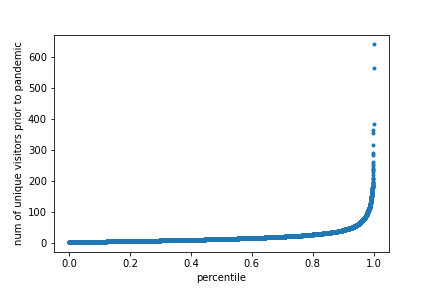
\includegraphics[width=0.8\textwidth, center]{./figures/1.percentile.png}
	\captionsetup{width=1.0\textwidth}
	\label{figure1}
	%\caption*{\footnotesize Each $a$--$b$ group shows impact of closure on grades completed by 2011 for children who were between $a$ and $b$ years of age at the time of school closure. These results correspond to results from column 1 of Table \ref{regone} which had 5 age-at-closure groups. 
\end{figure}

\begin{figure}[h]
	\centering
	\caption{\small Changes in average visitors in CA}
	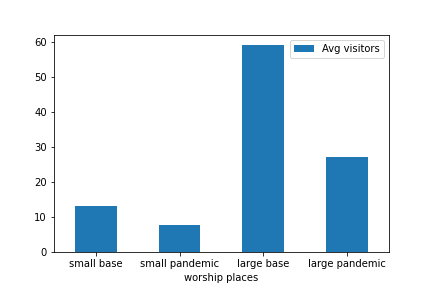
\includegraphics[width=0.8\textwidth, center]{./figures/avg_visit.png}
	\captionsetup{width=1.0\textwidth}
	\label{figure2}
	%\caption*{\footnotesize Each $a$--$b$ group shows impact of closure on grades completed by 2011 for children who were between $a$ and $b$ years of age at the time of school closure. These results correspond to results from column 1 of Table \ref{regone} which had 5 age-at-closure groups. 
\end{figure}


\begin{figure}[h]
	\centering
	\caption{\small Distribution of religious POIs in Alameda and San Francisco counties}
	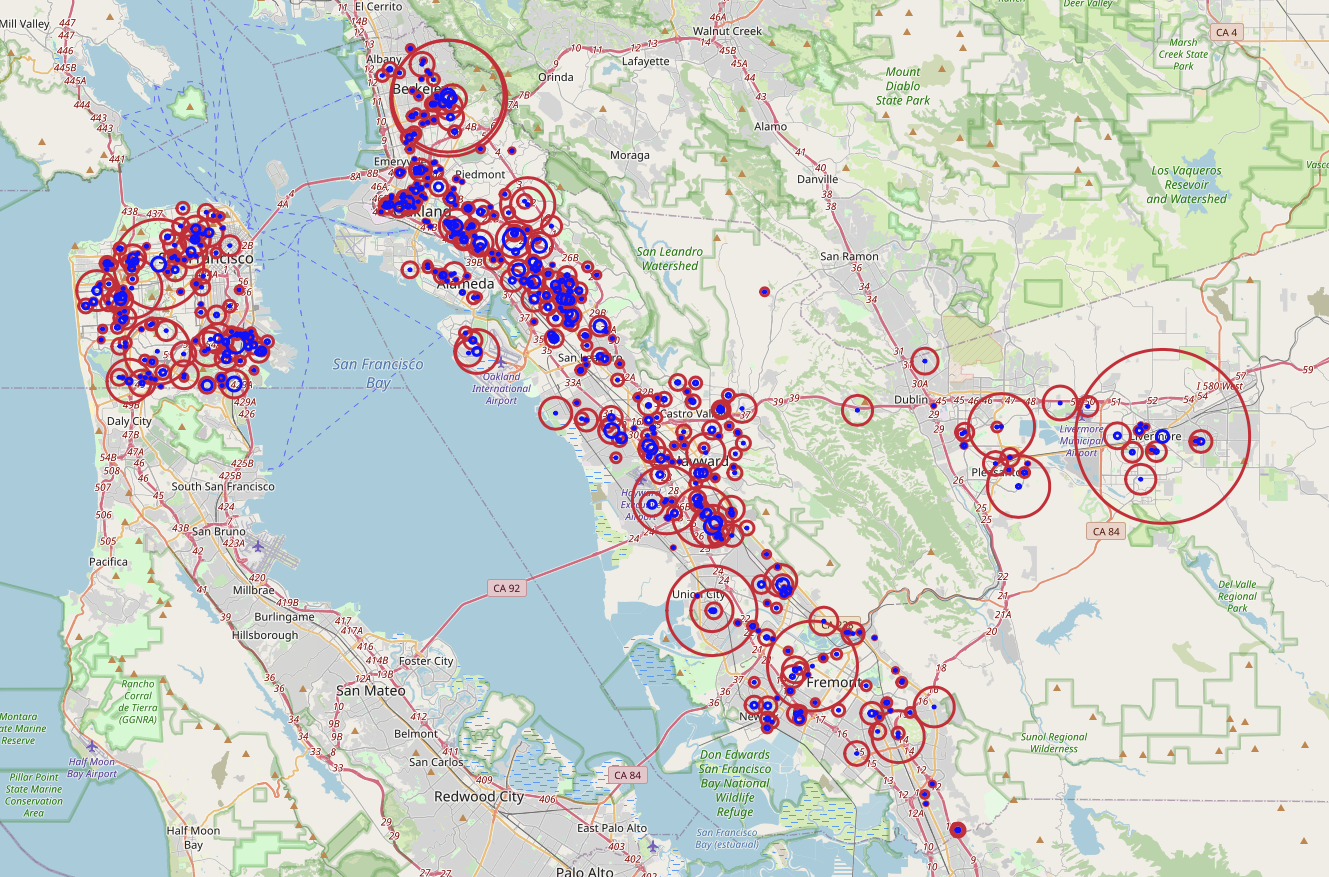
\includegraphics[width=0.85\textwidth, center]{./figures/2.POIs.png}
	\captionsetup{width=1.0\textwidth}
	\label{figure3}
	%\caption*{\footnotesize Each $a$--$b$ group shows impact of closure on grades completed by 2011 for children who were between $a$ and $b$ years of age at the time of school closure. These results correspond to results from column 1 of Table \ref{regone} which had 5 age-at-closure groups. 
\end{figure}




\pagebreak
\begingroup
\setstretch{1.0}
%\setstretch{1.1}
\setlength\bibitemsep{0pt}
%\printbibliography
\endgroup
\pagebreak




\end{document}

\begin{equation}
\label{eq:targetcost}
Z\left(\tau,\delta\right) =
\sum\limits_{
	\substack{
		\mathrm{cohort} \\ \in{\left\{70,72,74,76\right\}}}
}
\left\{\delta\cdot
\int_{\epsilon}
\int_{Y_{min}}^{F_{Y}^{-1}\left(\tau\right)}
\int_{X}
N\Big(
\substack{
	Y,X,\epsilon; \\
	\delta, \Gamma_{\mathrm{cohort}}
}
\Big)f\left(X|Y\right)f\left(Y\right)f\left(\epsilon\right)\mathrm{d}X\mathrm{d}Y\mathrm{d}\epsilon\right\}
\end{equation}

